\documentclass[11pt]{beamer}
\usepackage[utf8]{inputenc}
\usepackage{lmodern}
\usepackage[T2A]{fontenc}
\usepackage{cmbright}
\usepackage[russian]{babel}
\usetheme{Darmstadt}
\usepackage{amsmath}
\usepackage{amsfonts}
\usepackage{bm}
\usepackage{graphicx}
% Использовать полужирное начертание для векторов
\let\vec=\mathbf

\DeclareMathOperator{\mathspan}{span}
\DeclareMathOperator{\mathdim}{dim}
\DeclareMathOperator{\rank}{rank}
\DeclareMathOperator{\diag}{diag}
\begin{document}
	\author{Е. Ларин, Ф. Ежов, И. Кононыхин }
	\title{Обучение с учителем. Классификация. Дискриминантный анализ. }
	%\subtitle{}
	%\logo{}
	\institute{Санкт-Петербургский государственный университет 
		
		Прикладная математика и информатика
		
		Вычислительная стохастика и статистические модели
	}
	\date{}
	\subject{Семинар по статистическому и машинному обучению}
	\setbeamercovered{transparent}
	\setbeamertemplate{navigation symbols}{}
	\begin{frame}[plain]
		\maketitle 
	\end{frame}
	
	\begin{frame}
		\frametitle{Обучение с учителем}
		
		Выборка из генеральной случайной величины
		\begin{itemize}
			\item Для задачи регрессии: $\bm{X} \in \mathbb{R}^{n\times p}, \;\;\mathbf{y}\in \mathbb{R}^n$
		    \item Для задачи классификации: $\bm{X} \in \mathbb{R}^{n\times p}, \;\;\mathbf{y}\in \mathbb{A}^n$
        \end{itemize}
		
	\end{frame}
	\begin{frame}
		\frametitle{Обучение с учителем: формальная постановка}
		\begin{itemize}
			\item \textit{Вход}: $\bm{X}$ --- выборка $\bm{\xi}$, $\bm{y}$ --- выборка $\eta$. Предполагаем, что существует неизвестное отображение $y^*: \bm{\xi} \to \eta$  (гипотеза непрерывности или компактности)
			
			\item \textit{Задача}: По $\bm{X}$ и $\bm{y}$ найти такое отображение $\hat{y}^*: \bm{\xi} \to \eta$, которое приблизит отображение  $y^*$. 
			
			\item \textit{Оценка}: Функция потерь $\mathfrak{L}(y^*(x), \hat{y}^*(x))$. Здесь $x$ --- реализация $\bm{\xi}$
		\end{itemize}
	\end{frame}
	
	\begin{frame}
		\frametitle{Классификация}
		\begin{equation}
			\bm{X} \in \mathbb{R}^{n\times p}, \;\;\mathbf{y}\in \mathbb{A}^n
		\end{equation}
		\begin{block}{Гипотеза компактности}
			<<Близкие>> объекты, как правило, принадлежат одному классу
		\end{block}
		Понятие близости может быть формализовано, например, так:
		$$\rho(\bm{x_1}, \bm{x_2}) = \left(\displaystyle{\sum_{i = 1}^p w_i|x_1^i - x_2^i|^k}\right)^{{1}\over {k}}$$
	\end{frame}

	\begin{frame}
		\frametitle{Классификация: генеральная постановка}
		\textit{Дано:}
		\begin{itemize}
			\item $\bm{\xi} \in \mathbb{R}^p$ --- вектор признаков
			\item $\eta \in \mathbb{A}$ --- классовая принадлежность
		\end{itemize}
	
		Предположение об их зависимсти можно записать в виде \ref{2}.
		\begin{equation}
			\eta = \Phi(\bm{\xi}, \varepsilon)
			\label{2}
		\end{equation}
		Обычно на $\varepsilon$ накладываются условия $$E\varepsilon = 0, \;\; D\varepsilon = \sigma^2, \bm{\xi} \perp \varepsilon$$
		
		\textit{Задача:} найти $\Phi$
	\end{frame}
	\begin{frame}
		\frametitle{Классификация: выборочная постановка}
		\textit{Дано:}
		\begin{itemize}
			\item $\bm{X} \in \mathbb{R}^{n\times p}$ --- матрица признаков
			\item $\bm{y} \in \mathbb{A}^n$ --- вектор классовой принадлежности
		\end{itemize}
		
		Предположение имеет вид \ref{3}.
		\begin{equation}
			y_i = \Phi(\bm{x}_i, \varepsilon_i),\;\;\; i = 1, \ldots, n
			\label{3}
		\end{equation}
		
		\textit{Задача:} найти $\Phi$
	\end{frame}
	\begin{frame}
		\frametitle{Классификация: оценка качества}
		\begin{figure}
			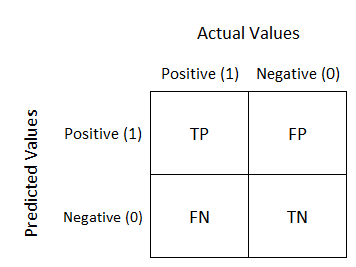
\includegraphics[width=0.3\linewidth]{imgs/conf_matrix}
		\end{figure}
	    На основе этой матрицы есть большое количество разных метрик: \textit{accuracy}, \textit{recall}, \textit{precision}, $F_\beta$, \textit{ROC--AUC}
	\end{frame}
	\begin{frame}
		\frametitle{Классификация: типы классов}
		\begin{itemize}
			\item По количеству классов:
			\begin{itemize}
				\item бинарная классификация
				\item многоклассовая классификация
			\end{itemize}
			\item По пересечению классов 
			\begin{itemize}
				\item пересекающиеся
				\item непересекающаяся
				\item нечёткие
			\end{itemize}
		\end{itemize}
	\end{frame}
	\begin{frame}
		\frametitle{Классификация: этапы обучения модели}
		\begin{itemize}
			\item Выбор модели (класс рассматриваемых $\Phi$ из \ref{3})
			\item Выбор метрики
			\item Выбор метода обучения (способ подбора параметров для минимизации метрики на обучающем множестве)
			\item Выбор метода проверки (способ оценки качества модели)
		\end{itemize}
	\end{frame}
	\begin{frame}
		\frametitle{Классификация: задача оптимизации}
		\begin{itemize}
			\item $\hat{\beta}$ --- параметры модели
			\item $\bm{\Phi}(\bm{x}, \beta)$ --- функционал классификации
			\item $\mathfrak{L}(\bm{\Phi}(\bm{x}, \beta), \bm{y})$ --- функция потерь (метрика)
		\end{itemize}
		\begin{block}{}
			$$\hat{\beta} = \arg\min_{\beta} \mathfrak{L}(\bm{\Phi}(\bm{x}, \beta), \bm{y})$$
		\end{block}
	
	\end{frame}
	\begin{frame}
		\frametitle{Классификация: общий подход к решению}
		Как построить функционал $\Phi$?
		
		
		Общий подход --- построить набор $f_i$, $i = 1, \ldots, K$. Каждая функция $f_i(\bm{x})$ показывает меру принадлежности $\bm{x}$ классу $i$. 
		
		Таким образом,
		\begin{equation}
			\Phi(\bm{x}) = \arg\max_i(f_i(\bm{x})).
			\label{4}
		\end{equation}
	\end{frame}
	\begin{frame}
		\frametitle{Дискриминантный анализ}
		Примем за функции $f_i$ из \ref{4} оценку вероятности принадлежности к $i$-му классу.
		
		$$\Phi(\bm{x}) = \arg\max_i (P(C_i|\bm{x})).$$
		
		$C_i$ ---  класс, состоящий из одного события: $\bm{x}$ принадлежит $i$-му классу.
	\end{frame}
	\begin{frame}
		\frametitle{Дискриминантный анализ}
		Если известны априорные вероятности получения $i$-го класса ($\pi_i$), применим формулу Байеса
		
		$$P(C_i|\bm{x}) = {{\pi_i P(\bm{x}|C_i)}\over{\sum_{j=1}^{K} \pi_j P(\bm{x}|C_j)}}.$$
		 
		 Отбросим знаменатель
		
		$$f_i = P(C_i|\bm{x}) = \pi_i P(\bm{x}|C_i).$$
	\end{frame}
	\begin{frame}
		\frametitle{LDA}
		\textit{Предположение:}	
		$$\mathtt{P}(\bm{\xi}|\eta = A_i) = \mathtt{N}(\bm{\mu}_i, \bm{\Sigma})$$
		
		\textit{Классифицирующая функция:}
		$$f_i(\bm{x}) = {{\pi_i}\over{(2\pi)^{p/2}|\bm{\Sigma}|^{1/2}}}exp\left(-{{1}\over{2}}(\bm{x} - \bm{\mu}_i)\bm{\Sigma}^{-1}(\bm{x} - \bm{\mu}_i)^\mathtt{T}\right)$$
		
		\textit{После упрощения:}
		$$h_i(\bm{x}) = -0.5 \bm{\mu}_i\bm{\Sigma}^{-1}\bm{\mu}_i^\mathtt{T} + \bm{\mu}_i\bm{\Sigma}^{-1}\bm{x} + \log\pi_i$$

	\end{frame}

	\begin{frame}
		\frametitle{QDA}
		\textit{Предположение:}	
		$$\mathtt{P}(\bm{\xi}|\eta = A_i) = \mathtt{N}(\bm{\mu}_i, \bm{\Sigma}_i)$$
		
		\textit{Классифицирующая функция:}
		$$f_i(\bm{x}) = {{\pi_i}\over{(2\pi)^{p/2}|\bm{\Sigma}_i|^{1/2}}}exp\left(-{{1}\over{2}}(\bm{x} - \bm{\mu}_i)\bm{\Sigma}_i^{-1}(\bm{x} - \bm{\mu}_i)^\mathtt{T}\right)$$
		
		\textit{После упрощения:}
		$$g_i(\bm{x}) = -0.5 (\bm{x} - \bm{\mu}_i)\bm{\Sigma}^{-1}(\bm{x} - \bm{\mu}_i)^\mathtt{T} - 0.5\log|\bm{\Sigma}_i| + \log\pi_i$$
		
	\end{frame}

	\begin{frame}
	\frametitle{Лог. регрессия}
			Зададим модель логистической регрессии следующим образом:
			% $$\bm{X} \in \mathbb{R}^{n\times p}, \;\;\mathbf{y}\in \mathbb{A}^n,$$
			$$\log \dfrac{P(\eta = G_i | \bm{\xi} = \bm{x})}{P(\eta = G_K | \bm{\xi} = \bm{x})} = \beta_{i0} + \bm{\beta}_{i}^T \bm{x}, i = 1, \cdots, K-1.$$
		
	\end{frame}
	\begin{frame}
		\frametitle{Лог. регрессия}
			Перейдем от логитов к вероятностям:
			
			$$P(\eta = G_i | \bm{\xi} = \bm{x})\ = \dfrac{e^{\beta_{i0} + \bm{\beta}_{i}^T \bm{x}} }{1 + \sum_{k = 1}^{K-1} e^{\beta_{k0} + \bm{\beta}_{k}^T \bm{x}}} , i = 1, \cdots, K-1 ,$$
			$$P(\eta = G_K | \bm{\xi} = \bm{x}) = \dfrac{1}{1 + \sum_{k = 1}^{K-1} e^{\beta_{k0} + \bm{\beta}_{k}^T \bm{x}}}.$$
	\end{frame}

	\begin{frame}
		\frametitle{Лог. регрессия: метод максимального правдоподобия}
		
		Для оценки параметров воспользуемся методом максимального правдоподобия:
		
			$$ l(\theta) = \sum\limits_{i=1}^{N} \log P(\eta = G_k | \bm{\xi} = \bm{x}; \theta ), $$
			$$ \theta = (\beta_{10}, \beta^T_1, \dotsc, \beta_{(K-1)0}, \beta^T_{K-1}). $$
		
		
		 Iteratively reweighted least squares (IRLS).
		
	\end{frame}

	\begin{frame}
	\frametitle{Лог. регрессия}
	
		Функция потерь.
		$$ L(M_i(\beta)) = \log(1 + e^{-y_i \beta^T x_i}) $$
		
	\end{frame}
\end{document}